\chapter{Introduction} \label{introduction}
\graphicspath{Figures/chapter1/}
\section{Graphs}
In this subsection, the main aspects of graph theory are briefly presented.
\subsection{Introduction}


% \subsubsection{Begginings and historical remarks}


% \subsubsection{Introduction}

In the real world, many problems can be described by a diagram connecting a set of points with
lines, joining pairs of these points, or even creating loops on a single point. A simple example
of that would be a set of points representing people with lines connecting acquintances, or
points representing atoms and lines representing chemical bonds, creating a representation of
a molecule as a graph attribute. In the examples above, the only information contained is whether
two points are associated, with the manner being disregarded. The concept of a graph consists of
a mathematical abstraction of the above. \cite{book:2008}


\begin{definition} \label{u_simple_graph} Mathematically, in its simplest form, a
  \textbf{graph} is an ordered pair\footnotemark{} $G=(V, E)$ of:
  \begin{itemize}
  \item \textbf{V}, a set of vertices (also known as nodes).
  \item $E \subseteq \{\{x, y\} | x,y \in V ~x \neq y \}$, which is the set of \textbf{edges}
    which consists of unordered pairs of vertices that connect two nodes.
  \end{itemize}
\footnotetext{An ordered pair $(a, b)$ is a pair of objects in which the order of
appearance or insertion is significant; the ordered pair $(a, b)$ is different than $(b,
a)$ unless $a=b$. An unordered pair is a set of the form ${a, b}$ is a set having two
elements with no relation between them and ${a, b} = {b, a}$.  }
\end{definition}

This type of object is called an \textbf{undirected simple graph} to avoid confusion
with other types.

\begin{definition}\label{graph_def}
  A \textit{graph} G is an ordered pair $(V(G), E(G))$ consisting of a set
$V(G)$ of \textit{vertices} (also called \textit{nodes} or \textit{points}) and a set
$E(G)$, disjoint from $V(G)$ which consists of \textit{edges} (also called \textit{links}
or \textit{lines}) together with an incidence function $\psi_G$ that associates with each
edge of G an unordered pair of not necesserily distinct vertices of G.  If $e$ is an edge
and $u$ and $v$ are vertices such that $\psi_G ={u, v}$ then $e$ is said to \textit{join}
$u$ and $v$, and the vertices $u$ and $v$ are called the \textit{ends} of $e$. We denote
the numbers of vertices and edges $G$ by $u(G)$ and $e(G)$ which two parameters are called
the \textit{order} and \textit{size} of G, respectively \cite{book:2008}.

  In short, we can define a \textbf{graph} as an ordered triple $G=(V, E, \phi_G)$
consisting of:
  \begin{itemize}
  \item $V$, a set of \textit{vertices}
  \item $E$, a set of \textit{edges}
  \item $\phi_G: E \rightarrow \{\{x, y\} | x, y \in V \; and \; x \neq y\}$ an
\textit{incidence function} mapping every edge to an unordered pair of vertices - an edge
associated with two distinct vertices. The incidence function is a function of the edges.
  \end{itemize} This type of object is called an \textit{undirected multigraph}, to avoid
confusion. Note, that the above definition of the \textit{incidence function} does not
allow for \textit{loops} (mappings of an edge on the same vertex).

A \textit{loop} is a an edge that allows a connection of a vertex to itself and a graph can
be defined to either allow or disallow the presence of loops. Some authors allow for loops
to exist on \textit{multigraphs} \cite{article:bollobas}, while other consider these kind
of graphs to exist in a different category, called \textit{pseudographs} \cite{book:Gary}.
Allowing loops requires modifying the incidence function so they can be supported. The new
incidence function can be written as:
\begin{equation}\label{eq:phi} \phi_G : E \rightarrow \{\{x, y \} | x,y \in V\} \end{equation}
The example presented below should better illustrate clarify the definition (of a pseudograph).
\begin{figure}[H]
  \begin{center}
  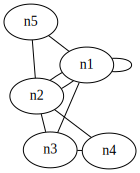
\includegraphics[scale=0.5]{Figures/chapter1/definition_ex_1.png}
\end{center}
  \caption{An undirected pseudograph with labeled nodes and
edges.}\label{fig:SimplePseudograph}

\end{figure}
\begin{example}

  \

For the graph presented in  \fref{fig:SimplePseudograph}  the following
can be assumed:
\begin{align*}
    &G = (V(G), E(G))
    &\intertext{and} 
    &V(G) = \{n_1, n_2, n_3, n_4, n_5\} \\
    &E(G) = \{A, B, C, D, E, F, G, H, I\} 
    &\intertext{and the incidence function is defined as:}
    &\psi_G(A) = n_1n_2,\quad \psi_G(B) = n_1n_2, \quad \psi_G(C) =
      n_1n_1, \quad \psi_G(D) = n_2n_3,\\
    &\psi_G(E) = n_1n_3, \quad \psi_G(F) = n_3n_4, \quad \psi_G(G) = n_2n_4,
      \quad \psi_G(H)= n_1n_5, \\
    &\psi_G(I) = n_2n_5
\end{align*}
\end{example}
  
It should now be clear that with the newer definition of $\phi_G$, self loops are now possible.
Additionaly, even though this was not prohibited by the previous definition, it is worth
noting that a node can be connected to another with multiple edges (or multiedges), or that it can have zero
connections to other nodes. Generally, $V$ is assumed to be a non-empty set, but $E$ can be
empty.

It is now possible to define some characteristic attributes of graphs:
\begin{itemize}
\item $|V|$: the \textbf{order} of a graph is the number of its vertices.
\item $|E|$: the \textbf{size} of a graph is the number of its edges.
\item The \textbf{degree} (or \textbf{valency}) of a single node is the number of
  edges connected to it. The \textbf{degree} of a graph is the maximum number of
  edges connected to a single vertex that belongs to it.
\item The edges of create a \textit{homogenous relation}\footnotemark{} $\sim$ on the vertices
  of the graph that is called \textbf{adjacency relation}; for each edge \textit{$(x, y)$}, its
  endpoints \textit{x, y} are said to be \textbf{adjacent} to each other, denoted by $x \sim y$.
  This property will be particulary useful when the adjacency matrix is defined in the following
  section.
\end{itemize}

\footnotetext{A \textbf{homogenous relation} (or \textbf{endorelation}) over a set \textit{X}
  is a set of assignments (binary relations) over \textit{X} and itself; i.e. it is a subset of
  the cartesian product $X\times X$
}

It can be inferred from the above definitions and attributes that for an undirected
graph of order \textit{n}, the maximum \textit{degree} of a node is $n~-~1$ and
and maximum \textit{size} of a graph is $n(n~-~1)/2$.

\end{definition}

In this section only \textit{undirected} graphs were considered, which are graphs
with edges with no orientation. A whole other class of graph objects with edges which
have orientation exists, called \textit{directed graphs}. These kind of graphs objects
are out of scope for this thesis and will not be presented.


\subsection{Adjacency Matrix}
\begin{definition}
  The \textit{adjacency matrix} is the fundamental mathematical representation of a graph.
  It is a square matrix, the elements of which represent which pair of nodes are
  \textit{adjacent} or not. Thus, the adjacency matrix \textbf{A} of a graph of order $n$
  is the $n\times n$ matrix with elements $A_{ij}$ such that:
  \begin{equation}
    \label{eq:adj_mat}
    A_{ij} = \begin{cases} 1 &\text{if there exists at least one edge connecting $i$ and $j$} \\
               0 &\text{if there no edges connecting those edges directly.}

             \end{cases}
\end{equation}
\end{definition}


\begin{figure}
     \begin{subfigure}[t]{0.4\textwidth}
         \centering
         \includegraphics[width=\textwidth]{Figures/chapter1/simple_graph_adj.png}
         \caption{Multigraph with no loops and multiple edges.}
         \label{fig:simple_adj_demo}
     \end{subfigure}
     \hfill
     \begin{subfigure}[t]{0.4\textwidth}
         \centering
         \includegraphics[width=\textwidth]{Figures/chapter1/complex_graph_adj.png}
         \caption{Mutligraph with loops and multiple edges.}
         \label{fig:compl_adj_demo}
     \end{subfigure}
        \caption{Two undirected multigraphs.}
        \label{fig:two multigraphs}
\end{figure}

Considering the simple undirected graph of \fref{fig:simple_adj_demo} we can construct
the following adjacency matrix:
\begin{table}[H]
  
  \begin{equation*}
    A = 
    \begin{pmatrix}
      0 & 1 & 1 & 0 & 1 & 0 \\
      1 & 0 & 1 & 1 & 1 & 1 \\
      1 & 1 & 0 & 1 & 0 & 0 \\
      0 & 1 & 1 & 0 & 0 & 0 \\
      1 & 1 & 0 & 0 & 0 & 0 \\
      0 & 1 & 0 & 0 & 0 & 0 
    \end{pmatrix}
  \end{equation*}
  \caption{Adjacency matrix for \fref{fig:simple_adj_demo}}
\end{table}

For this simple network, which has no loops and only one edge connect two nodes,
the diagonal matrix elements are always zero and the matrix is symmetric, as for
each edge connecting $i$ and $j$ there is a representation for the $j$ to $i$ connection
as well.

In a more complex case, such as the one presented in \fref{fig:compl_adj_demo} where loops
and multiedges are present an adjacency matrix can still be constructed. In this case,
a multiedge is represented by setting the value of the corresponding $A_{ij}$ value equal
to the multiplicity of the edge. In this case, $A_{12} = A_{21} = 2$.

For loops, the most common representation in the case of undirected
graphs is to still set the value of the $A_{ii}$ element equal to $2$
(i.e. $A_{11} = 2$ in the example presented).  Essentially, an edge of
a loop has two ends that connect to the same node, thus the result
\cite[p.~68]{book:algebraic}. Additionaly, defining the matrix in such
manner, allows for better computations and is consistent with the
definition of the representation of an edge connecting two nodes of an
undirected graph \cite[p.~108]{book:Newman}. 

Thus, the adjacency matrix for the graph of \fref{fig:compl_adj_demo} is

\begin{table}[H]
  \begin{equation*}
    A = 
   \begin{pmatrix}
      2 & 2 & 1 & 0 & 1 & 0 \\
      2 & 0 & 1 & 1 & 1 & 1 \\
      1 & 1 & 0 & 1 & 0 & 0 \\
      0 & 1 & 1 & 0 & 0 & 0 \\
      1 & 1 & 0 & 0 & 0 & 0 \\
      0 & 1 & 0 & 0 & 0 & 0 
    \end{pmatrix}
  \end{equation*}
  \caption{Adjacency matrix for  \fref{fig:compl_adj_demo}}
\end{table}

\begin{remark}
  Note that the degree of a node can be easily found by summing the values of
  the column or row of the adjacency matrix that correspond to said node.
\end{remark}
\subsubsection{Adjacency List}
  An alternative to the adjacency matrix is the \textit{adjacency
list}. An adjacency list is a collection of lists, one for each node
$i$. Each list contains the labels of the nodes that $i$ is connected
to, and its the most common method for storing networks on computers
as it requires less space. It is also possible to represent edge
attributes in an adjacency list by appending an extra column which
holds these values. An example for the graph presented in
\fref{fig:compl_adj_demo} with multiedges and loops:

\begin{table}[H]
  \centering
\begin{tabular}{|l|l|}
\hline
\rowcolor[HTML]{C0C0C0} 
{\color[HTML]{000000} Node} & {\color[HTML]{000000} Neighbors} \\ \hline
1                           & 1,2,2,5,3                        \\ \hline
2                           & 1,1,3,5,6,4                     \\ \hline
3                           & 1,2,4                           \\ \hline
4                           & 3,2                             \\ \hline
5                           & 1,2                             \\ \hline
6                           & 2                                \\ \hline
\end{tabular}
\label{table:adj_list_ex}
\caption{Adjacency list for \fref{fig:compl_adj_demo}}
\end{table}
Each edge of the network appears twice, thus for a network with $m$
edges the size of the adjacency list would be $2m$, much smaller
compared to the $n \times n$ matrix required to build an adjacency
matrix. This is particularly useful in networks which are relatively
\textit{sparse}\footnote{\textit{Sparse} networks are networks with a
much lower number of edges than those possible.}, but have a high
order.

\subsection{Graph Laplacian}\label{sec:laplacian}

The graph lacplacian is another representation matrix representation
of a graph. In its simplest form, for a simple, undirected and unweigheted
network of order $n$, is a $n \times n$ matrix \textbf{L} with elements:
\begin{equation*}
  L_{ij} = \begin{cases}k_i, &\text{if $i=j$}\\
             -1, & \text{if i $\neq$ j and there exists an edge connecting $i$ and $j$} \\
             0, & \text{everywhere else}
           \end{cases} 
\end{equation*}
where $k_i$ is the degree of the node. Another way to write the graph Lacplacian
is as
\begin{equation*}
  \textbf{L} = \textbf{D} - \textbf{A}
\end{equation*}
where \textbf{D} is a diagonal matrix containing the degrees of the nodes.

In a similar manner the Laplacian matrix can be constructed for weighted networks,
by replacing the the degree $k_i$ of a node with the relevant matrix elements.

The Laplacian matrix has many applications in the study of dynamical systems,
random walks and graph visualization. It has also found applications in graph
neural networks, as its spectral decomposition allows the construction of low
dimensional embeddings with applications in graph neural networks, such as
ChebNet \cite{article:ChebNet} which will be discussed in depth later.

\subsection{Edge weights} \label{sec:edge_weights}

So far, while presenting edges, we have considered graphs where
connections between nodes represented binary relations between them;
they either existed or they did not. In many situations when studying
graphs, it is useful to represent edges as connections which carry some
kind of attribute or value, commonly called \textit{weight}. This weight
could be any real number that fits a particular example, such as the distance
between two airfields on an airline network, the kinship of connections
on a social network (negative values can represent animosity and vice versa)
or any type of relational attribute that can be quantified and
characterizes the connection between nodes that belong in the same
network\cite[p.~109]{book:Newman}. A simple example is presented in
the figure below.
\begin{figure}[h]
     \begin{subfigure}[c]{0.4\textwidth}
         \centering
         \includegraphics[scale=0.5]{Figures/chapter1/simple_weighted.png}
         \caption{Multigraph with no loops and multiple edges.}
         \label{fig:simple_adj_demo}
     \end{subfigure}
     \hfill
     \begin{subfigure}[c]{0.4\textwidth}
       \centering
       \begin{equation*}
         A = 
        \begin{pmatrix}
        0 & 4 & 0.5 \\
        4 & 0 & 1.2 \\
        0.5 & 1.2 & 0 
        \end{pmatrix}  
\end{equation*}
\newline
\newline
\newline
\newline
\newline
\caption{Corresponding adjacency matrix.}
\label{table:weighted_adj}
\end{subfigure}
  \caption{Simple example of an unordered graph with weighted edges}
  \label{fig:weighted_graph}
\end{figure}

Generally, edges and nodes can hold any type of variable as values,
such as vectors, the usefulness of which will become apparent when
computer algorithms for graph representations and graph neural
networks are discussed in later sections and chapters.


\subsection{Distance between nodes and shortest paths}

On a graph, any route that traverses nodes along the edges connecting them
creates a sequence which is called a \textit{walk}. Walks are not prohibited
from traversing previously visited nodes and edges, but walks that do not intersect
themselves are called \textit{paths}.

\begin{remark}
  \textit{Adjacency Matrix Powers}  ~Before continuing, it is worth
  mentioning that the powers of the adjacency matrix $A^c$ directly provide
  the number of walks of length $c$ among two nodes. If there is a connection
  between two nodes $i$ and $j$, then $A_{ij} = 1$ else it is 0. Moving
  to the second power and taking for example an intermediate node $k$
  which might lie between $i$ and $j$, the product $A_{ik}{kj}$ would be
  1 if there is a node and 0 if there is not \cite[p.~131]{book:Newman}.
  Generalizing to walks of length $c$ which traverse nodes $i$ to $j$, their
total number is:
  \begin{equation*}
    N^{(c)}_{ij} = [A^c]_{ij}
  \end{equation*}
\end{remark}

The \textit{shortest path} between two nodes is the shortest walk
between those two nodes, the walk which traverses the least amount of
nodes. In terms of edges, the least number that must be traversed
is called \textit{shortest distance}
or often just ``distance''. Mathematically, the shortest distance
between two nodes $i$ and $j$ is the walk with the smallest value $c$ where
$[A^c]_{ij} > 0$

  \begin{example}
    For instance consider the following graph:
\begin{figure}[!h]
     \begin{subfigure}[c]{0.4\textwidth}
         \centering
         \includegraphics[scale=0.45]{Figures/chapter1/simple_graph_dist.png}
         % \label{fig:simple_adj_demo}
     \end{subfigure}
     \hfill
     \begin{subfigure}[c]{0.4\textwidth}
       \centering
       \begin{equation*}
         A = 
\begin{pmatrix}
0 & 1 & 1 & 0 & 1 & 0 \\
1 & 0 & 1 & 1 & 1 & 0 \\
1 & 1 & 0 & 0 & 0 & 0 \\
0 & 1 & 0 & 0 & 0 & 1 \\
1 & 1 & 0 & 0 & 0 & 0 \\
0 & 0 & 0 & 1 & 0 & 0 \\
 
\end{pmatrix} \end{equation*}
\label{table:weighted_adj}
\end{subfigure}
  \caption{A graph with a maximum path of 3 (nodes 1 to 6).}
  \label{fig:weighted_graph}
\end{figure}

In this example, it can be visiually determined that the minimum walk
between nodes 1 and 6 is of length 3.  Indeed, raising the adjacency
matrix to a power of three yields for these nodes:
\begin{equation*}
  \begin{split}
 &\cdots \\
 &N_{1,6}^{(2)} = \sum^nA_{1k}A_{k6} = [A^2]_{1,6} = 0 \\
 &N_{1,6}^{(3)} = \sum^nA_{1k}A_{kl}A_{l6} = [A^3]_{1,6} = 1
    \end{split}
\end{equation*}
  \end{example}


  

% The \textit{distance} between nodes is the number of edges that must be
% traversed to reach

\subsection{Node and edge properties}
  As mentioned in \sref{sec:edge_weights}, edges can hold more information
  than just the binary relations between nodes. In fact, this concept can
  be generalized to nodes and even whole graphs. When studying graphs and
  networks, especially when using computational methods for applications
  like complex dynamics, it is the most natural way to phrase data on a
  graph. The data can be any real number or even categorical data, such
  as colors.

  The matrices which hold the information mentioned before are
  \begin{itemize}
  \item \textbf{V: vertex (or node) attributes} (i.e. a label or
number of neighbors)
  \item \textbf{E: edge (or link) attributes} (i.e. a label or edge
weight)
  \item \textbf{U: global (or master node) attributes} (i.e. number of
nodes or number of paths of length 2)
  \end{itemize}

  Global attributes usually get their values as an aggregation of the
  attributes of the nodes and edges, and methods applied on them.
  For instance, a molecule might have chemical elements as node
  attributes, types of bonds as edge attributes and the toxicity of
  the molecule as graph attributes.  An example of a classroom should
  better illustrate the concept.
\newpage

  

  \begin{example}
    In this example, a classroom of 5 classmates is presented. Each student
    has a number of \textbf{node} attributes, their age, heigh and average
    grade (from F to A). \textbf{Edge} attributes between students hold
    information about their physical proximity when seated for class,
    and their kinship (as a real number between $0-1$). Finally,
    \textbf{global} attributes consist of information about the classroom,
    such as total number of students and class's failure rate.
    \begin{figure}[!h]
     \begin{subfigure}[c]{0.4\textwidth}
         \centering
         \includegraphics[scale=0.45]{Figures/chapter1/example_node_properties.png}
     \end{subfigure}
     \hfill
     \begin{subfigure}[c]{0.4\textwidth}
       \centering
       \begin{equation*}
         A = 
\begin{pmatrix}
0 & 1 & 0 & 0 & 1 \\
1 & 0 & 1 & 0 & 1 \\
0 & 1 & 0 & 1 & 1 \\
0 & 0 & 1 & 0 & 1 \\
1 & 1 & 1 & 1 & 0 \\ 
\end{pmatrix} \end{equation*}
\label{table:properties_example}
\end{subfigure}
  \caption{Example graph of a small classroom with labeled edges and nodes}
  \label{fig:properties_example}
\end{figure}

\begin{table}[h]%
  \centering
  \subfloat[][]{
\begin{tabular}{|
>{\columncolor[HTML]{C0C0C0}}l |l|l|l|}
\hline
Node & \cellcolor[HTML]{C0C0C0}Age & \cellcolor[HTML]{C0C0C0}Height & \cellcolor[HTML]{C0C0C0}Grade \\ \hline
s1   & 11.5                        & 135                            & C                             \\ \hline
s2   & 12                          & 140                            & B                             \\ \hline
s3   & 12                          & 142                            & A                             \\ \hline
s4   & 11.5                        & 132                            & A                             \\ \hline
s5   & 12                          & 143                            & B                             \\ \hline
\end{tabular}}
  \qquad
  \subfloat[][]{
    \begin{tabular}{|
>{\columncolor[HTML]{C0C0C0}}l |l|l|}
\hline
Edge & \cellcolor[HTML]{C0C0C0}Distance & \cellcolor[HTML]{C0C0C0}Kinship \\ \hline
A    & 1.5                              & 0.5                             \\ \hline
B    & 1.2                              & 0.5                             \\ \hline
C    & 0.5                              & 0.8                             \\ \hline
D    & 2                                & 0.35                            \\ \hline
E    & 2                                & 0.3                             \\ \hline
F    & 0.5                              & 0.9                             \\ \hline
\end{tabular}
  }
  \caption{A) Node properties B) Edge properties}%
  \label{tbl:Node and edge properties}%
\end{table}
\begin{table}[h!]
  \centering
\begin{tabular}{|l|l|l|}
\hline
\rowcolor[HTML]{C0C0C0} 
                          & No. Nodes & Failure \% \\ \hline
\cellcolor[HTML]{C0C0C0}G & 5         & 0          \\ \hline
\end{tabular}
\caption{Graph Properties}
\end{table}

\end{example}

\clearpage
\section{Network Dynamics}

Frequently, it is useful to consider cases where the status of the
networks studied changes over time. This could mean that the topology
of the network changes (i.e. nodes and edges are added or removed),
the internal state of the network changes (the properties discussed in
the previous section) or both. 

The main concern of this thesis is with networks with a fixed topology
, but with elements (nodes and edges) whose properties constitute
dynamical quantities which can change over time. Following some dynamical
rule, nodes can interact with their neighbors or change their own
properties, with edges dictating which interactions are possible.
In fact, the study of network dynamics combines graph theory with
non-linear dynamics \cite{book:Jost2007}.

For many real world situations, a proper model of their processes
consists of dynamical systems acting on networks. This can range
from opinion spreading, epidemics, flow of electricity on grids,
spread of packages on internet networks and many more systems
whose dynamics are evolving on a network. In fact, many network
processes can be understood 